% Created by tikzDevice version 0.6.2-92-0ad2792 on 2013-10-13 23:59:58
% !TEX encoding = UTF-8 Unicode
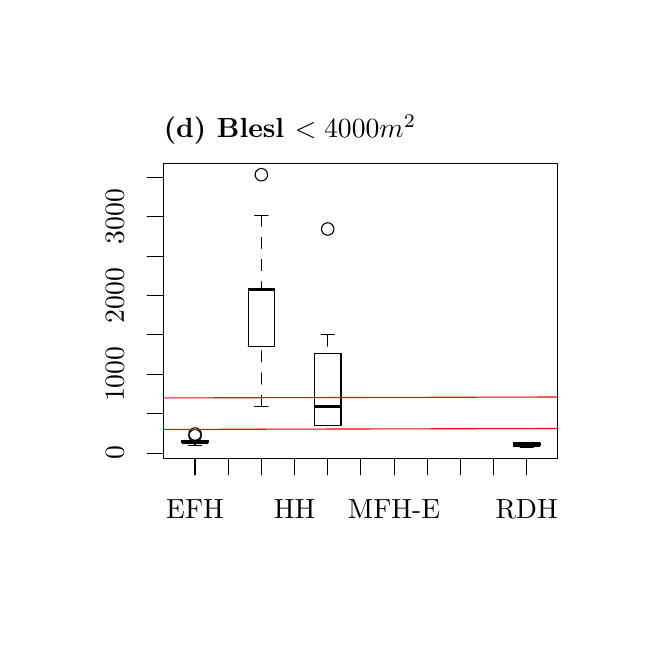
\begin{tikzpicture}[x=1pt,y=1pt]
\definecolor[named]{fillColor}{rgb}{1.00,1.00,1.00}
\path[use as bounding box,fill=fillColor,fill opacity=0.00] (0,0) rectangle (216.81,216.81);
\begin{scope}
\path[clip] ( 49.20, 61.20) rectangle (191.61,167.61);
\definecolor[named]{drawColor}{rgb}{0.00,0.00,0.00}

\path[draw=drawColor,line width= 1.2pt,line join=round] ( 55.67, 67.13) -- ( 65.26, 67.13);

\path[draw=drawColor,line width= 0.4pt,dash pattern=on 4pt off 4pt ,line join=round,line cap=round] ( 60.47, 65.97) -- ( 60.47, 66.91);

\path[draw=drawColor,line width= 0.4pt,dash pattern=on 4pt off 4pt ,line join=round,line cap=round] ( 60.47, 67.67) -- ( 60.47, 67.67);

\path[draw=drawColor,line width= 0.4pt,line join=round,line cap=round] ( 58.07, 65.97) -- ( 62.87, 65.97);

\path[draw=drawColor,line width= 0.4pt,line join=round,line cap=round] ( 58.07, 67.67) -- ( 62.87, 67.67);

\path[draw=drawColor,line width= 0.4pt,line join=round,line cap=round] ( 55.67, 66.91) --
	( 65.26, 66.91) --
	( 65.26, 67.67) --
	( 55.67, 67.67) --
	( 55.67, 66.91);

\path[draw=drawColor,line width= 0.4pt,line join=round,line cap=round] ( 60.47, 69.35) circle (  2.25);

\path[draw=drawColor,line width= 0.4pt,line join=round,line cap=round] ( 60.47, 69.98) circle (  2.25);

\path[draw=drawColor,line width= 1.2pt,line join=round] ( 79.65,122.15) -- ( 89.24,122.15);

\path[draw=drawColor,line width= 0.4pt,dash pattern=on 4pt off 4pt ,line join=round,line cap=round] ( 84.44, 80.03) -- ( 84.44,101.48);

\path[draw=drawColor,line width= 0.4pt,dash pattern=on 4pt off 4pt ,line join=round,line cap=round] ( 84.44,149.04) -- ( 84.44,122.15);

\path[draw=drawColor,line width= 0.4pt,line join=round,line cap=round] ( 82.05, 80.03) -- ( 86.84, 80.03);

\path[draw=drawColor,line width= 0.4pt,line join=round,line cap=round] ( 82.05,149.04) -- ( 86.84,149.04);

\path[draw=drawColor,line width= 0.4pt,line join=round,line cap=round] ( 79.65,101.48) --
	( 89.24,101.48) --
	( 89.24,122.15) --
	( 79.65,122.15) --
	( 79.65,101.48);

\path[draw=drawColor,line width= 0.4pt,line join=round,line cap=round] ( 84.44,163.67) circle (  2.25);

\path[draw=drawColor,line width= 1.2pt,line join=round] (103.62, 80.03) -- (113.21, 80.03);

\path[draw=drawColor,line width= 0.4pt,dash pattern=on 4pt off 4pt ,line join=round,line cap=round] (108.42, 73.02) -- (108.42, 73.08);

\path[draw=drawColor,line width= 0.4pt,dash pattern=on 4pt off 4pt ,line join=round,line cap=round] (108.42,105.78) -- (108.42, 99.04);

\path[draw=drawColor,line width= 0.4pt,line join=round,line cap=round] (106.02, 73.02) -- (110.82, 73.02);

\path[draw=drawColor,line width= 0.4pt,line join=round,line cap=round] (106.02,105.78) -- (110.82,105.78);

\path[draw=drawColor,line width= 0.4pt,line join=round,line cap=round] (103.62, 73.08) --
	(113.21, 73.08) --
	(113.21, 99.04) --
	(103.62, 99.04) --
	(103.62, 73.08);

\path[draw=drawColor,line width= 0.4pt,line join=round,line cap=round] (108.42,144.06) circle (  2.25);

\path[draw=drawColor,line width= 1.2pt,line join=round] (175.55, 66.02) -- (185.14, 66.02);

\path[draw=drawColor,line width= 0.4pt,dash pattern=on 4pt off 4pt ,line join=round,line cap=round] (180.34, 65.14) -- (180.34, 65.85);

\path[draw=drawColor,line width= 0.4pt,dash pattern=on 4pt off 4pt ,line join=round,line cap=round] (180.34, 66.96) -- (180.34, 66.73);

\path[draw=drawColor,line width= 0.4pt,line join=round,line cap=round] (177.94, 65.14) -- (182.74, 65.14);

\path[draw=drawColor,line width= 0.4pt,line join=round,line cap=round] (177.94, 66.96) -- (182.74, 66.96);

\path[draw=drawColor,line width= 0.4pt,line join=round,line cap=round] (175.55, 65.85) --
	(185.14, 65.85) --
	(185.14, 66.73) --
	(175.55, 66.73) --
	(175.55, 65.85);
\end{scope}
\begin{scope}
\path[clip] (  0.00,  0.00) rectangle (216.81,216.81);
\definecolor[named]{drawColor}{rgb}{0.00,0.00,0.00}

\path[draw=drawColor,line width= 0.4pt,line join=round,line cap=round] ( 60.47, 61.20) -- (180.34, 61.20);

\path[draw=drawColor,line width= 0.4pt,line join=round,line cap=round] ( 60.47, 61.20) -- ( 60.47, 55.20);

\path[draw=drawColor,line width= 0.4pt,line join=round,line cap=round] ( 72.46, 61.20) -- ( 72.46, 55.20);

\path[draw=drawColor,line width= 0.4pt,line join=round,line cap=round] ( 84.44, 61.20) -- ( 84.44, 55.20);

\path[draw=drawColor,line width= 0.4pt,line join=round,line cap=round] ( 96.43, 61.20) -- ( 96.43, 55.20);

\path[draw=drawColor,line width= 0.4pt,line join=round,line cap=round] (108.42, 61.20) -- (108.42, 55.20);

\path[draw=drawColor,line width= 0.4pt,line join=round,line cap=round] (120.41, 61.20) -- (120.41, 55.20);

\path[draw=drawColor,line width= 0.4pt,line join=round,line cap=round] (132.39, 61.20) -- (132.39, 55.20);

\path[draw=drawColor,line width= 0.4pt,line join=round,line cap=round] (144.38, 61.20) -- (144.38, 55.20);

\path[draw=drawColor,line width= 0.4pt,line join=round,line cap=round] (156.37, 61.20) -- (156.37, 55.20);

\path[draw=drawColor,line width= 0.4pt,line join=round,line cap=round] (168.35, 61.20) -- (168.35, 55.20);

\path[draw=drawColor,line width= 0.4pt,line join=round,line cap=round] (180.34, 61.20) -- (180.34, 55.20);

\node[text=drawColor,anchor=base,inner sep=0pt, outer sep=0pt, scale=  1.00] at ( 60.47, 39.60) {EFH};

\node[text=drawColor,anchor=base,inner sep=0pt, outer sep=0pt, scale=  1.00] at ( 96.43, 39.60) {HH};

\node[text=drawColor,anchor=base,inner sep=0pt, outer sep=0pt, scale=  1.00] at (132.39, 39.60) {MFH-E};

\node[text=drawColor,anchor=base,inner sep=0pt, outer sep=0pt, scale=  1.00] at (180.34, 39.60) {RDH};

\path[draw=drawColor,line width= 0.4pt,line join=round,line cap=round] ( 49.20, 63.09) -- ( 49.20,162.70);

\path[draw=drawColor,line width= 0.4pt,line join=round,line cap=round] ( 49.20, 63.09) -- ( 43.20, 63.09);

\path[draw=drawColor,line width= 0.4pt,line join=round,line cap=round] ( 49.20, 77.32) -- ( 43.20, 77.32);

\path[draw=drawColor,line width= 0.4pt,line join=round,line cap=round] ( 49.20, 91.55) -- ( 43.20, 91.55);

\path[draw=drawColor,line width= 0.4pt,line join=round,line cap=round] ( 49.20,105.78) -- ( 43.20,105.78);

\path[draw=drawColor,line width= 0.4pt,line join=round,line cap=round] ( 49.20,120.01) -- ( 43.20,120.01);

\path[draw=drawColor,line width= 0.4pt,line join=round,line cap=round] ( 49.20,134.24) -- ( 43.20,134.24);

\path[draw=drawColor,line width= 0.4pt,line join=round,line cap=round] ( 49.20,148.47) -- ( 43.20,148.47);

\path[draw=drawColor,line width= 0.4pt,line join=round,line cap=round] ( 49.20,162.70) -- ( 43.20,162.70);

\node[text=drawColor,rotate= 90.00,anchor=base,inner sep=0pt, outer sep=0pt, scale=  1.00] at ( 34.80, 63.09) {0};

\node[text=drawColor,rotate= 90.00,anchor=base,inner sep=0pt, outer sep=0pt, scale=  1.00] at ( 34.80, 91.55) {1000};

\node[text=drawColor,rotate= 90.00,anchor=base,inner sep=0pt, outer sep=0pt, scale=  1.00] at ( 34.80,120.01) {2000};

\node[text=drawColor,rotate= 90.00,anchor=base,inner sep=0pt, outer sep=0pt, scale=  1.00] at ( 34.80,148.47) {3000};

\node[text=drawColor,anchor=west, inner sep=0pt, outer sep=0pt, scale=  1.00]
at (49.20,180) {\textbf{(d) Blesl $< 4000 m^2$}
\label{fig:AreaIWUheA}
};

\path[draw=drawColor,line width= 0.4pt,line join=round,line cap=round] ( 49.20, 61.20) --
	(191.61, 61.20) --
	(191.61,167.61) --
	( 49.20,167.61) --
	( 49.20, 61.20);
\end{scope}
\begin{scope}
\path[clip] ( 49.20, 61.20) rectangle (191.61,167.61);
\definecolor[named]{drawColor}{rgb}{1.00,0.00,0.00}

\path[draw=drawColor,line width= 0.4pt,line join=round,line cap=round] ( 49.20, 71.63) -- (191.61, 71.97);

\path[draw=drawColor,line width= 0.4pt,line join=round,line cap=round] ( 49.20, 83.02) -- (191.61, 83.35);
\end{scope}
<<<<<<< HEAD
\end{tikzpicture}
=======
\end{tikzpicture}
>>>>>>> 36a956db0f2ffb15b4b8091da9293464a1b25a0c